\section{Experimental Results}\label{sec:exp}

In this section be briefly describe our experimental setup, then provide some performance data on the JIT compiler itself, i.e. how fast is it, and finally we compare the code produced from the JIT compiler with the conventionally optimized and compiled code.

\mypar{Experimental setup}

All measurements were performed on a Intel Core i7-3632QM (Ivy Bridge) processor running a clock frequency of 3.2 GHz with cache sizes of 32kB (L1 data), 256kB (L2) and 6MB (L3). The clang compiler version 3.5 was used for all measurements with optimization flags: \texttt{-O3 -march=native}.

For the particle system itself we have seen a nearly non-existing influence from the number of particles. When going from a small particle set that fits into the first level cache to a multi GB set the effect on the overall runtime is around one or two additional cpu cycles per particle and therefore can simply be ignored for any practical purpose. This behaviour is mostly possible due to the perfect sequential traversal over the particles, the therefore perfect data access pattern for the hardware prefetcher, and the high enough computational load for most scenarios masking the memory accesses.
%~ Specify the platform (processor, frequency, cache sizes)
%~ as well as the compiler, version, and flags used. I strongly recommend that you play with optimization flags and consider also icc for additional potential speedup.


\mypar{JIT Compiler}

\begin{figure}[t]\centering
  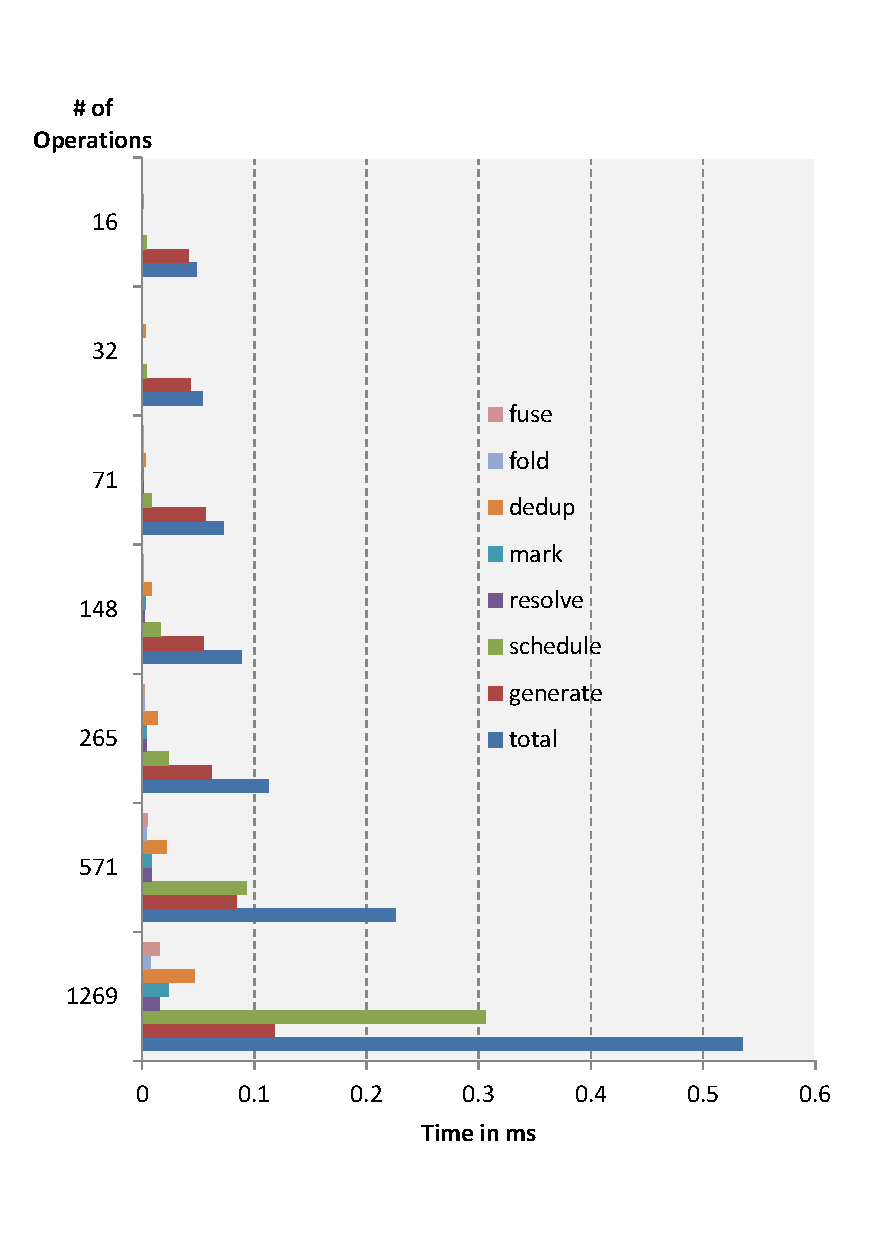
\includegraphics[width=0.5\textwidth]{jit_perf.pdf}
  \caption{Performance of the JIT compiler itself
  \label{perf_jit}}
\end{figure}

First we consider the performance of the JIT compiler itself. While compilation speed was not our primary concern we still have to make sure it is suited for real time usage. Meaning we want compilation times to be at least in the low milisecond range. For reference, the time budget to calculate a single update cycle in real time graphics tasks is typically 8-30 milisecond.
If we take a look at where the jit compiler spends its time [\ref{perf_jit}] we immediately see that all except two stages run in the range of a few microseconds and only the scheduling and code generation take significantly more time. The code generation runs in approximately constant time, around 40 to 120 microseconds, where most of the time is used for two system-calls. These two calls, \texttt{mmap} and \texttt{mprotect}, cause page faults and context switches within the operating system and therefore impose a constant cost that is hard to avoid. The actual writing of the code is only a minor part of the generation stage. Turning our attention to the scheduling stage we immediately see that the time used for the scheduling steps is strongly dependant on the number of rules, and by extension the number of instructions within them, that are composed together. For only a few rules the scheduling is still eclipsed by the code generation, for any at least mildly complex scenario though the scheduling does take a longer time to complete its work. Still the whole JIT compiler runs in the sub-millisecond range for reasonable use cases and is therefore fast enough for real time usage.

\mypar{Code Perfomance}

When looking at the performance of the code itself we distinguish two situations. The first one encompasses scenarios were there is only one or two rules and allows us to see how well our JIT compiler performs in direct comparison with AOT compilers. The second scenario takes a closer look at simulations with at least four and up to more than twenty rules, exhibiting the potential for optimizations across multiple rules. Before we go to these results here the list of what the different configurations in the plots represent
\begin{itemize}
\item naive: the naive implementation in SSA form
\item vector sse: implemented 3D-vector math in sse instructions
\item parallel sse 1: parallel processing of four particles without unrolling particles batches
\item parallel sse 8: parallel processing of four particles with 8-fold particle batches unrolled
\item jit scalar: the naive implementation as produced by the jit compiler by emitting scalar operations only
\item jit sse: vectorized code form the jit compiler using 128bit vector register, i.e processing 4 particles in parallel
\item jit avx: vectorized code from the jit compiler using the new 256bit register introduced with intel AVX extensions
\end{itemize}

\begin{figure}[th]\centering
  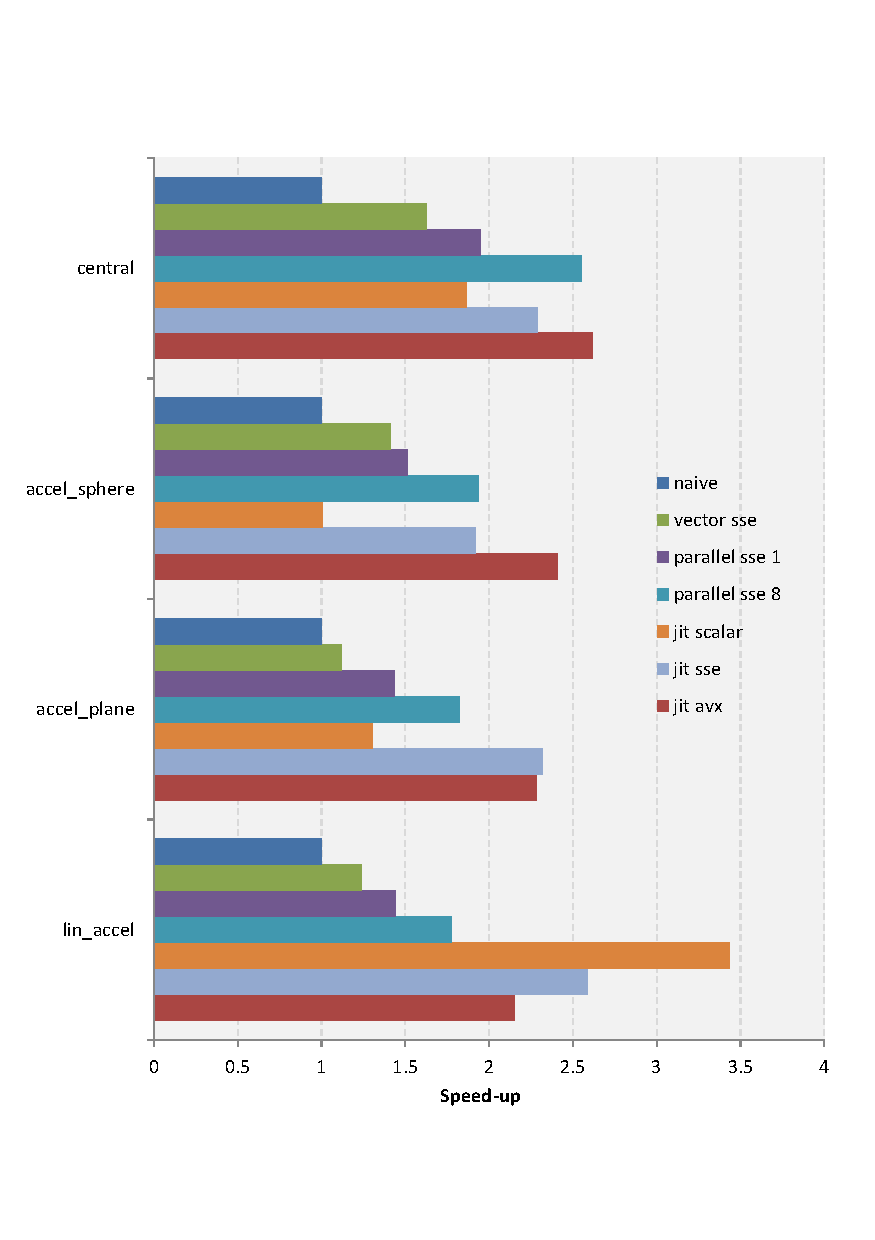
\includegraphics[scale=0.6]{single_dual_rules.pdf}
  \caption{Performance comparison for single or dual rule scenarios
  \label{perf_single}}
\end{figure}

Looking at figure \ref{perf_single} we can see that both our jit compiled and hand optimized code outperform the naive implementation to varying degrees. Due to required data shuffling neither can fully realize the theoretical speed up from vector instructions. In general we see the jit compiled code to be at least equally as fast as the conventional code. Also note that going from 4-way to 8-way vector instructions does not yield significant speed ups and in some cases even results in slow downs. This may be in part caused by added data shuffling. Some instructions (\texttt{sqrtps} and \texttt{divps} specifically) also have twice the latency and half the throughput in their 256bit versions on the used processor. Therefore they do not provide an actual advantage over their 128bit counterparts. The test cases called \emph{central4} and \emph{central8} in figure \ref{perf_multi} are strongly affected by this since their running time is dominated by those two instructions.

\begin{figure}[th]\centering
  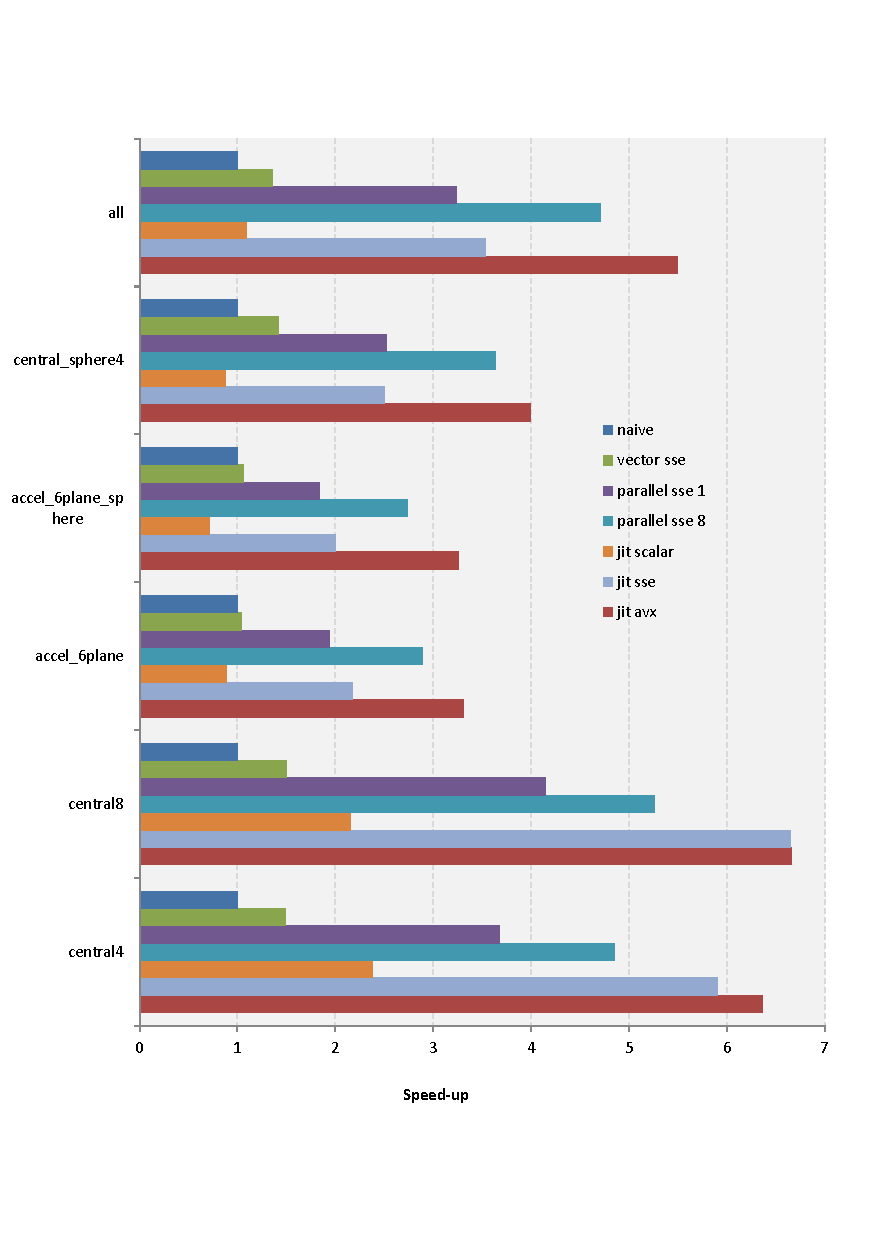
\includegraphics[scale=0.6]{multi_rules.pdf}
  \caption{Performance comparison for multi rule scenarios
  \label{perf_multi}}
\end{figure}

The test cases shown in figure \ref{perf_multi} use more rules at once and we see the results shift in favour of both optimization paths, with an advantage for out JIT compiler. For both the jit compiled and conventional code the presence of many rules and therefore operations allows to mask the required data shuffling we have seen in the previous comparison. Looking closely at the results we can see that the \texttt{jit avx} code always outperforms every other version, and the \texttt{jit sse} code outperfoming the equivalent hand optimized code, \texttt{parallel sse 1}, as well. Comparing the two conventionally optimized code versions \texttt{parallel sse 1} and \texttt{parallel sse 8} it is clear that the further loop unrolling done in the later is worth the effort, even if the instructions present in the multiple rules all but exhaust the instruction buffers on the cpu and such further unrolling does not provide obvious advantages.

One of the main advantages of the jit compiler is that it significantly reduces the amount of actually generated instructions. The optimization passes eliminate up to half of the instructions present in the input rules. Due to the types of optimizations that are performed it does however not reduce the critical path length. So the total latency of one loop iteration assuming perfect instruction level paralellism is unaffected. This reinforces the observation that loop unrolling could provide a speed up for the jit compiled code by allowing more efficient interleaving of independent paths of execution.



